\setcounter{chapter}{-1}
\setchapterpreamble[u]{\margintoc}
\chapter{The Helmholtz equation}
\label{h:helmholz}

In this introductory chapter, we will review the Helmholtz equation, as it is fundamental in photonics, and will be used in many of the subsequent chapters.

\sectionyoutubeugent{Maxwell's equations in the frequency domain}{Rx6ptGNSuKA}

\begin{marginfigure}[+0.0cm]
  % credits: Wikipedia
  % url: https://en.wikipedia.org/wiki/James_Clerk_Maxwell#/media/File:James_Clerk_Maxwell.png
  \includegraphics{helmholtz/figures/james_clerk_maxwell}
  \caption{James Clerk Maxwell}
\end{marginfigure}

To start with, let's recall Maxwell's curl equations in the time domain. In the absence of current sources, they are given by

\begin{equation}
\nabla \times {\mathbf E} ({\mathbf r},t) = - \mu({\mathbf r)} \frac{\partial {\mathbf H} ({\mathbf r} ,t)}{\partial t} \label{eq-rot-E}
\end{equation}
\begin{equation}
\nabla \times {\mathbf H} ({\mathbf r},t) = \varepsilon({\mathbf r}) \frac{\partial {\mathbf E}({\mathbf r},t)}{\partial t} \label{eq-rot-H}
\end{equation}

For the common case of linear isotropic media, the dielectric permittivity $\varepsilon$ and the magnetic permeability $\mu$ are scalars, which can however be a function of the spatial coordinate ${\mathbf r}$.

In the next chapters, we will restrict ourselves to the important case where all the fields have a harmonic time dependence with a fixed frequency $\omega$, e.g. for the $x$--component of the electric field:

\begin{equation}
E_x({\mathbf r},t) = E_{x,0}({\mathbf r}) \cos \left( \omega t + \phi_{E_x} ({\mathbf r})
\right) \label{eq-phasor}
\end{equation}

Similar expressions can be written for the other field components and for the magnetic field. It is convenient to introduce a complex number $\tilde{E}_x$ called a \emph{phasor}, that is defined as

\begin{equation}
\tilde{E}_x(\mathbf{r})=E_{x,0}({\mathbf r}) e^{j \phi_{E_x}({\mathbf r})} \label{eq:phasor}
\end{equation}

\begin{cue}
Given such a complex-valued phasor, how can we recover the real-valued electric field?
\end{cue}

\noindent\marginnote{Note that some people use a different convention, which results in $e^{-j \omega t}$. This can give rise to some surprising sign changes in formulas, so be aware of this!}The relation between the phasor and the electric field is given by

\begin{equation}
E_x({\mathbf r},t) = \Re \left(\tilde{E}_x({\mathbf r}) e^{j \omega t}\right)
\end{equation}

\begin{cue}
What is the phasor corresponding to $\partial E_x({\mathbf r},t) / \partial t$ ?
\end{cue}

By taking the time derivative of Eq.~\ref{eq-phasor}, it is easy to show that 

\begin{equation}
\frac{\partial E_x({\mathbf r},t)}{\partial t} = \Re \left(j \omega \tilde{E}_x({\mathbf r}) e^{j \omega t}\right)
\end{equation}

Therefore, the phasor corresponding to $\partial E_x({\mathbf r},t) / \partial t$ is given by $j \omega \tilde{E}_x({\mathbf r})$.

In what follows, we will omit the tilde and implicitly assume that we are always dealing with phasors. We can also collect the phasors for all field components in complex vectors ${\mathbf E}$ and ${\mathbf H}$. 

\begin{cue}
Write Eq.~\ref{eq-rot-E} and \ref{eq-rot-H} using phasor notation.
\end{cue}

Using phasor notation, Eq.~\ref{eq-rot-E} and \ref{eq-rot-H} become

\begin{equation}
\nabla \times {\mathbf E}({\mathbf r}) = - j \omega \mu({\mathbf r}) {\mathbf H}({\mathbf r})
\label{eq-rot-E-phas}
\end{equation}
\begin{equation}   
\nabla \times {\mathbf H}({\mathbf r}) = j \omega \varepsilon({\mathbf r}) {\mathbf E}({\mathbf r}) \label{eq-rot-H-phas}
\end{equation}

These are Maxwell's equations expressed in the frequency domain.

\begin{exer}
  % difficulty: trivial
  % ugent
  What phasor corresponds to time integration of $\tilde{E}_x$?
  \begin{sol}
    Answer goes here
  \end{sol}
  \begin{hnt}
    Hint goes here
  \end{hnt}
\end{exer}

\begin{exer}
  % difficulty: trivial
 How do you need to change Eq.~\ref{eq-phasor}, so that the time dependence of a phasor corresponds to $e^{-j \omega t}$? 
\end{exer}

\section{The Helmholtz equation}

\begin{cue}
Take the curl of Eq.~\ref{eq-rot-E-phas} and use Eq.~\ref{eq-rot-H-phas}.
\end{cue}

By taking the curl of Eq.~\ref{eq-rot-E-phas} and plugging Eq.~\ref{eq-rot-H-phas} in the result, we get

\begin{equation}
  \nabla \times \nabla \times {\mathbf E}({\mathbf r}) = \omega^2 \varepsilon({\mathbf r}) \mu({\mathbf r}) {\mathbf E}({\mathbf r})
  \label{eq-helm-1}
\end{equation}

From vector calculus we know that

\begin{equation}
\nabla \times \nabla \times {\mathbf E}({\mathbf r}) = \nabla (\nabla \cdot {\mathbf E}({\mathbf r})) - \nabla^2 {\mathbf E}({\mathbf r})
\end{equation}

\begin{cue}
Use this to simplify Eq. \ref{eq-helm-1} in a uniform medium without charge $\rho$. 
\end{cue}

Let's for the moment consider a uniform medium without charge $\rho$. In that case, Maxwell's divergence laws tell us that $\nabla \cdot {\mathbf E}({\mathbf r})=0$, leading to

\begin{equation}
\nabla^2 {\mathbf E}({\mathbf r}) + k^2 {\mathbf E}({\mathbf r}) = 0 \label{eq-helmholtz}
\end{equation}

where we have introduced the wave vector $k=\omega \sqrt{\varepsilon \mu}$.

Eq.~\ref{eq-helmholtz} is called the (vectorial) Helmholtz equation. Note that the same equation can also be derived for the magnetic field ${\mathbf H}$. In Cartesian coordinates, each of the vectorial components of ${\mathbf E}$ and ${\mathbf H}$ satisfy a scalar Helmholtz equation:

\begin{marginfigure}[-0.0cm]
  % credits: Wikipedia
  % url: https://en.wikipedia.org/wiki/Hermann_von_Helmholtz#/media/File:Hermann_von_Helmholtz.jpg
  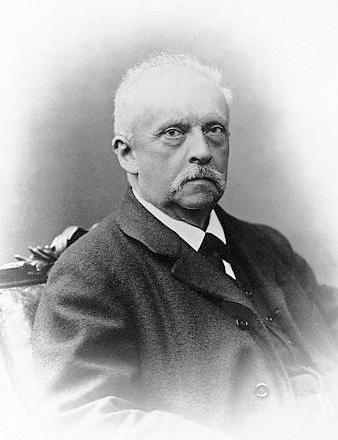
\includegraphics{helmholtz/figures/Hermann_von_Helmholtz}
  \caption{Hermann von Helmholtz}
\end{marginfigure}

\begin{equation}
\nabla^2 \psi({\mathbf r}) + k^2 \psi({\mathbf r}) = 0 \label{eq-helmholtz-1}
\end{equation}

Now, if we are studying a system which has a piecewise constant refractive index, Eq.~\ref{eq-helmholtz-1} will be valid in each of the uniform subregions. So formally we can write for the scalar Helmholtz equation in a medium with discrete index jumps:

\begin{equation}
\fbox{$\displaystyle \nabla^2 \psi({\mathbf r}) + k_0^2 n^2({\mathbf r}) \psi({\mathbf r}) = 0
\label{eq-helmholtz-3}$}
\end{equation}

Here, $k_0=\omega \sqrt{\varepsilon_0 \mu_0}$ is the wave vector in vacuum, and the refractive index $n$ is defined by $n=\sqrt{\varepsilon \mu} \sqrt{\varepsilon_0 \mu_0}$.

Eq.~\ref{eq-helmholtz-3} is strictly speaking only valid \emph{inside} each uniform subregion. At the interface between different media we still have to deal with the appropriate continuity conditions for the fields.

Since $\psi$ is a complex number, it seems worthwhile to study the calculus of functions of a complex variable. We will see that this has a number of direct applications in photonics, e.g. the Kramers--Kronig dispersion relations, and the use of conformal transformations to study waveguide bends.

\begin{exer}
    % difficulty: trivial
Solve the Helmholtz equation in a single uniform medium.
\end{exer}

\begin{exer}
    % difficulty: trivial
What does the Helmholz equation look like in case we use the time convention  $e^{-j \omega t}$? 
\end{exer}

\begin{exer}
      % difficulty: hard
The Helmholtz equation we derived here is only valid for uniform media. Exactly which step of the derivation breaks down in non-uniform media?
\end{exer}

\section*{Review questions}

\begin{itemize}
\item What is a phasor?
\item Write down Maxwell's curl equations in the frequency domain.
\item Write down the Helmholtz equation.
\end{itemize}



%%% Local Variables:
%%% mode: latex
%%% TeX-master: "../main"
%%% End:
